\documentclass[a11paper]{article}

\usepackage{karnaugh-map}
\usepackage{tabularx}
\usepackage{titlepage}
\usepackage{document}
\usepackage{booktabs}
\usepackage{multicol}
\usepackage{float}
\usepackage{varwidth}
% \usepackage[toc,page]{appendix}
\usepackage[usenames,dvipsnames]{xcolor}

\title{Rapport d'APP}

\class{Logique Combinatoire}
\classnb{GEN420 \& GEN430}

\teacher{Marwan Besrour \& Gabriel Bélanger}

\author{
  \addtolength{\tabcolsep}{-0.4em}
  \begin{tabular}{rcl} % Ajouter des auteurs au besoin
      Benjamin Chausse & -- & CHAB1704 \\
      Shawn Couture    & -- & COUS1912 \\
  \end{tabular}
}

\newcommand{\todo}[1]{\begin{color}{Red}\textbf{TODO:} #1\end{color}}
\newcommand{\note}[1]{\begin{color}{Orange}\textbf{NOTE:} #1\end{color}}
\newcommand{\fixme}[1]{\begin{color}{Fuchsia}\textbf{FIXME:} #1\end{color}}
\newcommand{\question}[1]{\begin{color}{ForestGreen}\textbf{QUESTION:} #1\end{color}}

\begin{document}
\maketitle
\newpage
\tableofcontents
\newpage

\todo{test} \fixme{another test} \note{interesting} \question{wtf}

\section{Module thermo2bin}

\subsection{Démarche}
Le but était de convertir un code thermométrique de 12 bits en binaire 4 bits non signé. Hors, le nombre afficher par ce genre de code
est connue en comptant le nombre de bits à un. Donc, les équations logiques doivent compter le nombre de bit à 1. Le code étant 12 bits,
il a pu être divisé en trois sections de 4 bits ce qui a permis l'utilisation de tableaux de Karnaugh pour trouver les équations. Selon
la table de vérité (\todo{\ref{tab:table-de-vérité-thermométrique-4-bits}}) d'un code thermométrique de 4 bits, le bit le plus significatif
du résultat en binaire n'est jamais à 1. L'équation du bit $E$ est donc simplement $E=0$. Le bit $F$ est uniquement à 1 si $A$ est à un, donc
l'équation est simplement $F=A$. On a donc besoin des tables pour uniquement deux bits des 4. Les deux tables de karnaugh pour chaque bits
se retrouvent dans l'annexe (\todo{\ref{tab:karnaugh-bit-G}}, \todo{\ref{tab:karnaugh-bit-H}}). Uniquement l'équation du bit $H$ à eut une
simplification ou $A'$ à été mis en évidence. Les équations étant assez simplifié sont les suivantes:

\begin{align}
  E &= 0 \\ F &= A \\ G &= A'C \\ H &= A'(C'D+BC)
\end{align}

Après, les trois nombre binaires sont additionner ensemble pour obtenir un résultat correspondant au nombre de bits à 1 dans le code
thermométrique en utilisant des additionneur 4 bits. Pour ce qui est du code d'erreur, une validation par groupe de 2 bits qui s'occuppe
de s'assurer que le "LSB" n'est pas à 0 si le "MSB" est à un, sur tout les groupe de 2 bits consécutif permet de savoir rapidement s'il
y a des erreurs. (voir le code en annexe).

\subsection{Explication des schéma blocs}
Thermo2bin est composé de deux additionneur 4 bits, lesquels sont composé de 4 additionneur 1 bits. L'additionneur 1 bit fait avec de la
logique combinatoire et celui fait avec des commandes "cases" sont synthéthisé par Vivado et donne le même circuit. On retrouve dans le
module thermométrique 3 sections identiques de convertions thermométrique 4 bits en binaire non signé. Le module thermométrique à aussi
une section de détection d'erreur qui prend l'entrée directement.

\subsection{Fréquence d'opération}
Pour connaitre la fréquence d'opération maximum, on doit d'abord analyzer le schéma et trouver le plus long chemin qu'une entrée peut
parcourir avant d'arrivé à la sortie. Ceci peut être fait en regardant simplement les schémas créé par Vivado. Cependant, Vivado éxecute
une synthèse du circuit, fesant une optimisation des portes logiques et donc réduisant le nombre utilisé pour le module thermo2bin.

\subsection{Implémentation}

\section{Simulation Complète}

\section{Démarche d'analyse de compatibilité}
La première étape à été d'analyser le signal d'entrée de la carte thermométrique. La DEL 2 est connecté au connecteur JD1 en
configuration "pull-up". Ceci dit, il faut donc avoir un 0 logique à son entrée pour l'allumé. Cependant, trois inverseurs sont
connecté en série avant elle. Soit deux 74V1T04STR et un NC7SP04P5X alimenté à +1.2 Volts. Après analyse de $V_{OH}$, $V_{OL}$, $V_{IL}$
et $V_{IH}$ des deux portes logiques, le NC7SP04P5X à un $V_{OH}$ de maximum 1.1 volts tandis que le 74V1T04STR à besoin d'un $V_{IH}$
minimum de 2 Volts. Donc selon le 74V1T04STR, le NC7SP04P5X envoie toujours un niveau logique bas, ce qui résulte à une del
tout le temps allumé sauf lorsque le connecteur de test de la del est en mode de test car un bon niveau logique haut est envoyé à
l'entrée des 74V1T04STR.

\newpage
\appendix
\section{Code VHDL}
\todo{Finish this this}

\begin{figure}[H]
	\tiny
	\centering
	\begin{varwidth}{\linewidth}
		\begin{verbatim}
architecture Behavioral of Thermo2Bin is
    signal first_segment_of_four : STD_LOGIC_VECTOR(3 downto 0);
    signal second_segment_of_four : STD_LOGIC_VECTOR(3 downto 0);
    signal third_segment_of_four : STD_LOGIC_VECTOR(3 downto 0);

    component Add4Bits is
        Port ( A : in STD_LOGIC_VECTOR (3 downto 0);
            B : in STD_LOGIC_VECTOR (3 downto 0);
            C : in STD_LOGIC;
            R : out STD_LOGIC_VECTOR (3 downto 0);
            Rc : out STD_LOGIC);
    end component;

    signal first_plus_second : STD_LOGIC_VECTOR(3 downto 0);
    signal carry_out_first_plus_second : STD_LOGIC;
    signal last_carry_out : STD_LOGIC;

begin
    first_segment_of_four(3) <= '0';
    first_segment_of_four(2) <= thermo_bus(11);
    first_segment_of_four(1) <= NOT thermo_bus(11) AND thermo_bus(9);
    first_segment_of_four(0) <= NOT thermo_bus(11) AND ((NOT thermo_bus(9) AND thermo_bus(8)) OR (thermo_bus(10) AND thermo_bus(9)));

    second_segment_of_four(3) <= '0';
    second_segment_of_four(2) <= thermo_bus(7);
    second_segment_of_four(1) <= NOT thermo_bus(7) AND thermo_bus(5);
    second_segment_of_four(0) <= NOT thermo_bus(7) AND ((NOT thermo_bus(5) AND thermo_bus(4)) OR (thermo_bus(6) AND thermo_bus(5)));

    third_segment_of_four(3) <= '0';
    third_segment_of_four(2) <= thermo_bus(3);
    third_segment_of_four(1) <= NOT thermo_bus(3) AND thermo_bus(1);
    third_segment_of_four(0) <= NOT thermo_bus(3) AND ((NOT thermo_bus(1) AND thermo_bus(0)) OR (thermo_bus(2) AND thermo_bus(1)));

    first_plus_second_adder : Add4Bits port map (
      A => first_segment_of_four,
      B => second_segment_of_four,
      R => first_plus_second,
      Rc => carry_out_first_plus_second,
      C => '0');

    plus_third_adder : Add4Bits port map (
      A => first_plus_second,
      B => third_segment_of_four,
      R => binary_out,
      Rc => last_carry_out,
      C => carry_out_first_plus_second);

    error <= (
    (thermo_bus(11) AND NOT thermo_bus(10)) OR
    (thermo_bus(10) AND NOT thermo_bus(9)) OR
    (thermo_bus(9)  AND NOT thermo_bus(8)) OR
    (thermo_bus(8)  AND NOT thermo_bus(7)) OR
    (thermo_bus(7)  AND NOT thermo_bus(6)) OR
    (thermo_bus(6)  AND NOT thermo_bus(5)) OR
    (thermo_bus(5)  AND NOT thermo_bus(4)) OR
    (thermo_bus(4)  AND NOT thermo_bus(3)) OR
    (thermo_bus(3)  AND NOT thermo_bus(2)) OR
    (thermo_bus(2)  AND NOT thermo_bus(1)) OR
    (thermo_bus(1)  AND NOT thermo_bus(0)));

end Behavioral;
\end{verbatim}

	\end{varwidth}
	\caption{Module Thermo2bin}
\end{figure}

\begin{figure}[H]
	\tiny
	\centering
	\begin{varwidth}{\linewidth}
		\begin{verbatim}
architecture Behavioral of Add4Bits is

  signal bufA : STD_LOGIC;
  signal bufB : STD_LOGIC;
  signal bufC : STD_LOGIC;

  component Add1BitA is Port (
    X : in STD_LOGIC;
    Y : in STD_LOGIC;
    Ci: in STD_LOGIC;
    O : out STD_LOGIC;
    Co: out STD_LOGIC);
  end component;

  component Add1BitB is Port (
    X : in STD_LOGIC;
    Y : in STD_LOGIC;
    Ci: in STD_LOGIC;
    O : out STD_LOGIC;
    Co: out STD_LOGIC);
  end component;

begin

  first : Add1BitB port map (
    X  => A(0),
    Y  => B(0),
    Ci => C,
    O => R(0),
    Co => bufA);

  sec : Add1BitB port map (
    X  => A(1),
    Y  => B(1),
    Ci => bufA,
    O => R(1),
    Co => bufB);

  third : Add1BitA port map (
    X  => A(2),
    Y  => B(2),
    Ci => bufB,
    O => R(2),
    Co => bufC);

  fourth : Add1BitA port map (
    X  => A(3),
    Y  => B(3),
    Ci => bufC,
    O => R(3),
    Co => Rc);

end Behavioral;
\end{verbatim}

	\end{varwidth}
	\caption{Module Add4Bits}
\end{figure}

\begin{figure}[H]
	\tiny
	\centering
	\begin{varwidth}{\linewidth}
		\begin{verbatim}
architecture Behavioral of Add1BitA is

begin

  O  <= (X xor Y) xor Ci;
  Co <= ((X xor Y) and Ci) or (X and Y);

end;
\end{verbatim}

	\end{varwidth}
	\caption{Module Add1BitA}
\end{figure}

\begin{figure}[H]
	\tiny
	\centering
	\begin{varwidth}{\linewidth}
		\begin{verbatim}
architecture Behavioral of Add1BitB is

begin

Adder: process(X, Y, Ci) is variable buf: STD_LOGIC_VECTOR(2 downto 0);
begin
  buf(0) := X;
  buf(1) := Y;
  buf(2) := Ci;

  case (buf) is
    when "000" =>
      O  <= '0';
      Co <= '0';
    when "001" =>
      O  <= '1';
      Co <= '0';
    when "010" =>
      O  <= '1';
      Co <= '0';
    when "011" =>
      O  <= '0';
      Co <= '1';
    when "100" =>
      O  <= '1';
      Co <= '0';
    when "101" =>
      O  <= '0';
      Co <= '1';
    when "110" =>
      O  <= '0';
      Co <= '1';
    when "111" =>
      O  <= '1';
      Co <= '1';
    when others =>
      O  <= '0';
      Co <= '0';
  end case;

end process Adder;

end Behavioral;
\end{verbatim}

	\end{varwidth}
	\caption{Module Add1BitB}
\end{figure}

\section{Schémas Bloc}

\todo{Simulations}


\begin{figure}[H]
	\centering
	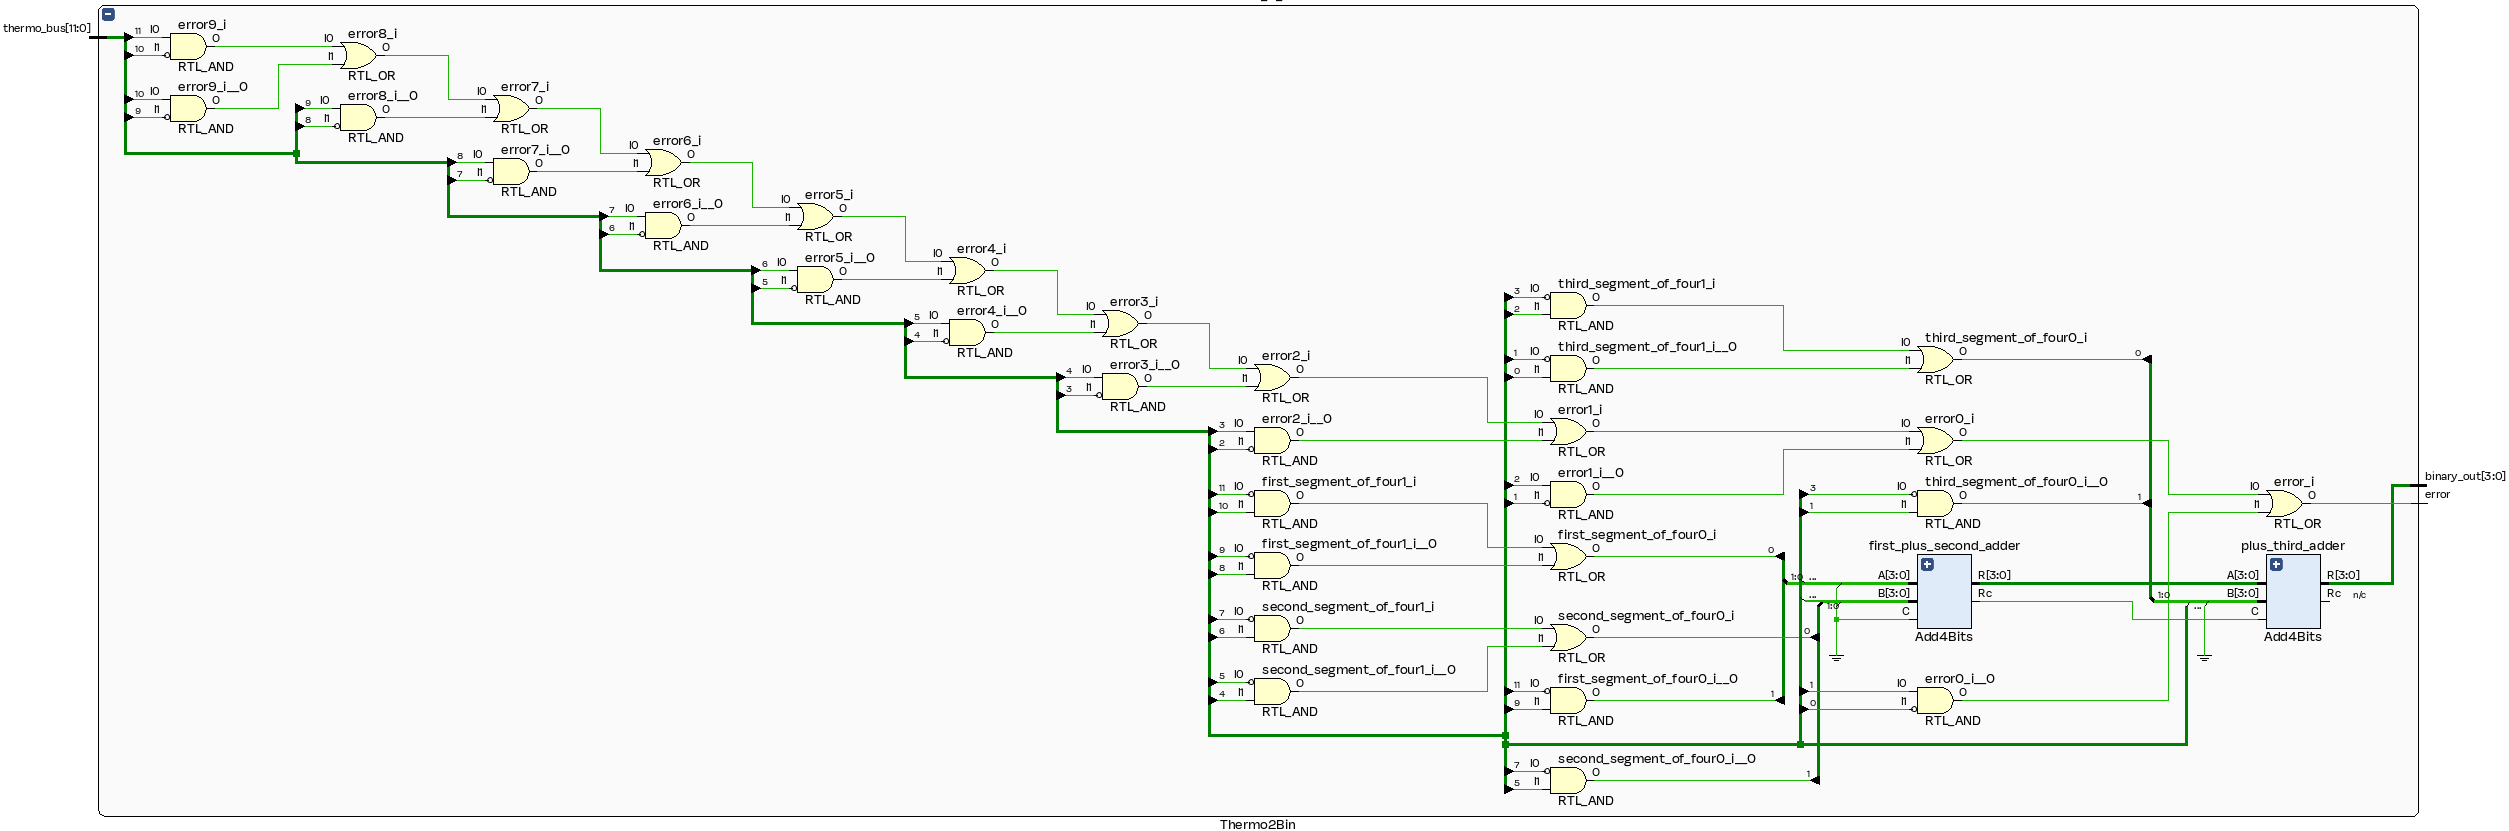
\includegraphics[width=\textwidth]{assets/img/schematic-thermo2bin.png}
	\caption{Module Thermo2bin}
\end{figure}

\begin{figure}[H]
	\centering
	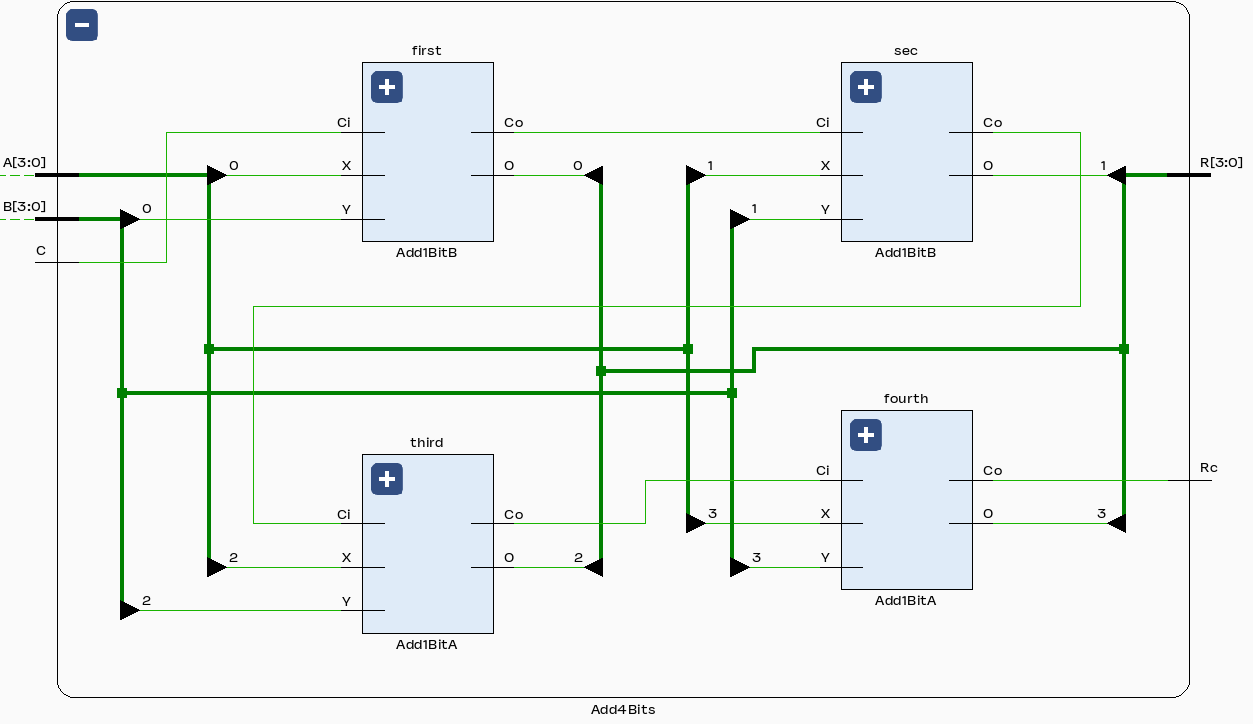
\includegraphics[width=.6\textwidth]{assets/img/schematic-add4bits.png}
	\caption{Module Add4Bits}
\end{figure}

\begin{figure}[H]
	\centering
	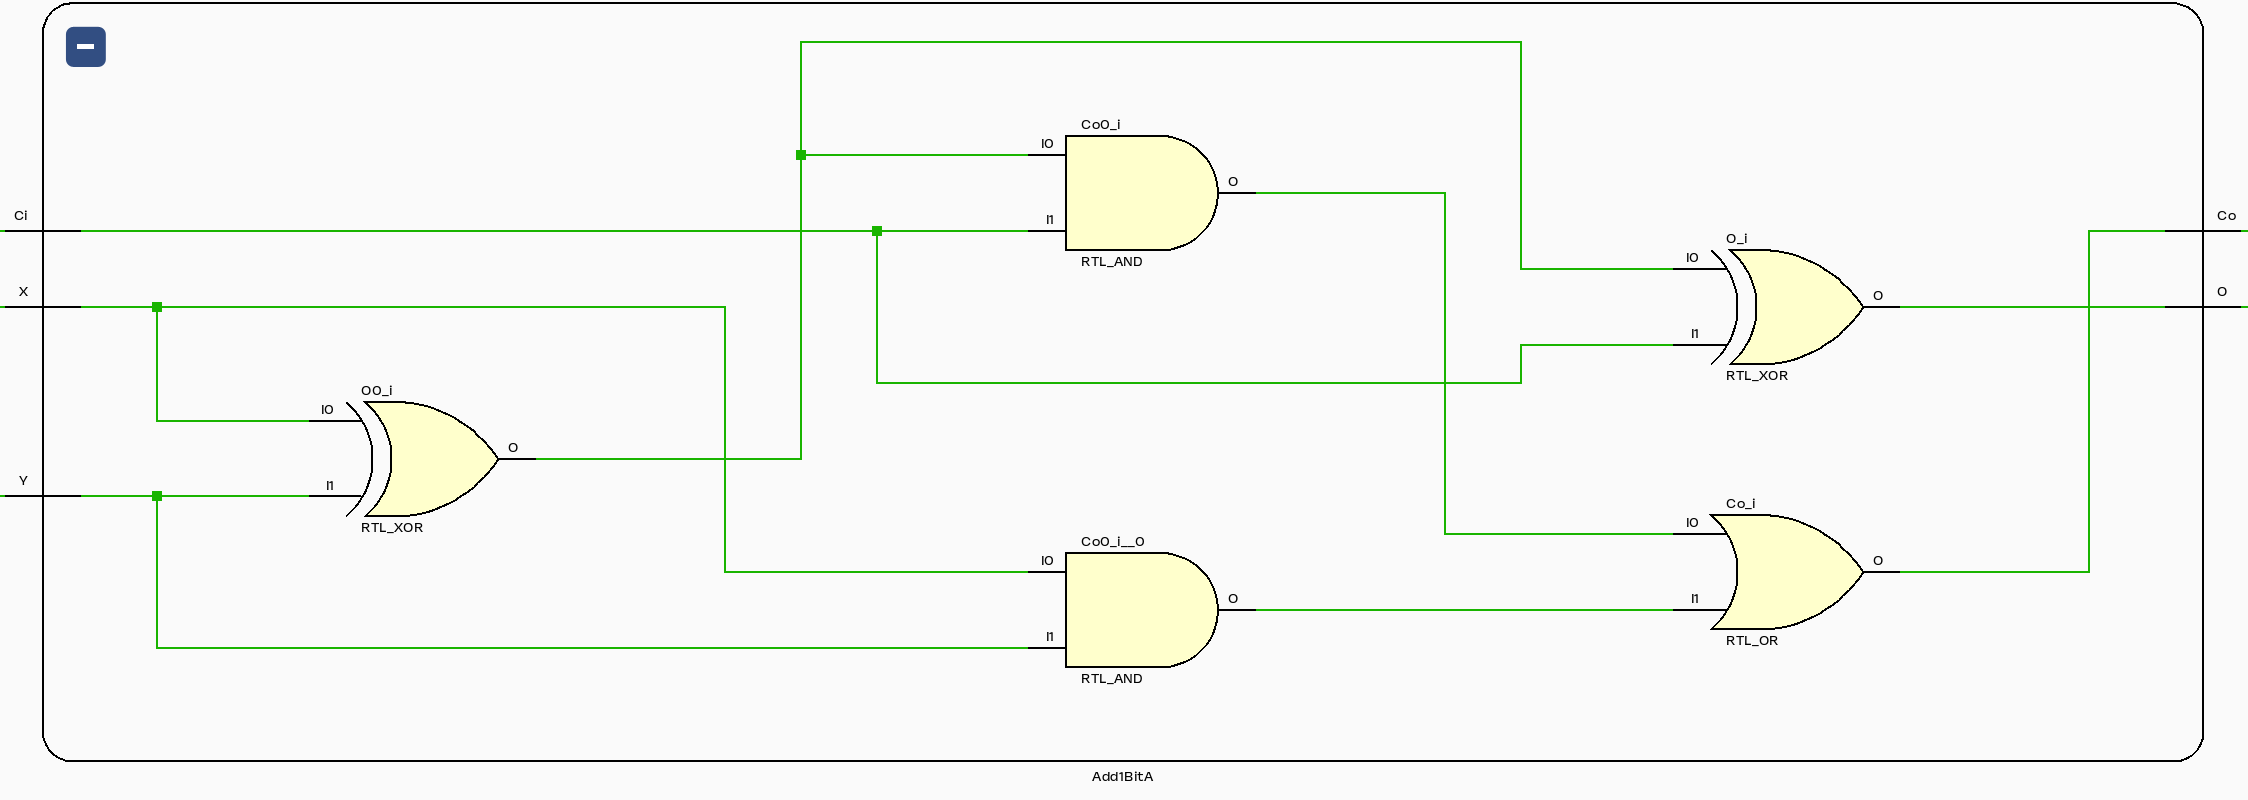
\includegraphics[width=.6\textwidth]{assets/img/schematic-add1bita.png}
	\caption{Module Add1BitA}
\end{figure}

\begin{figure}[H]
	\centering
	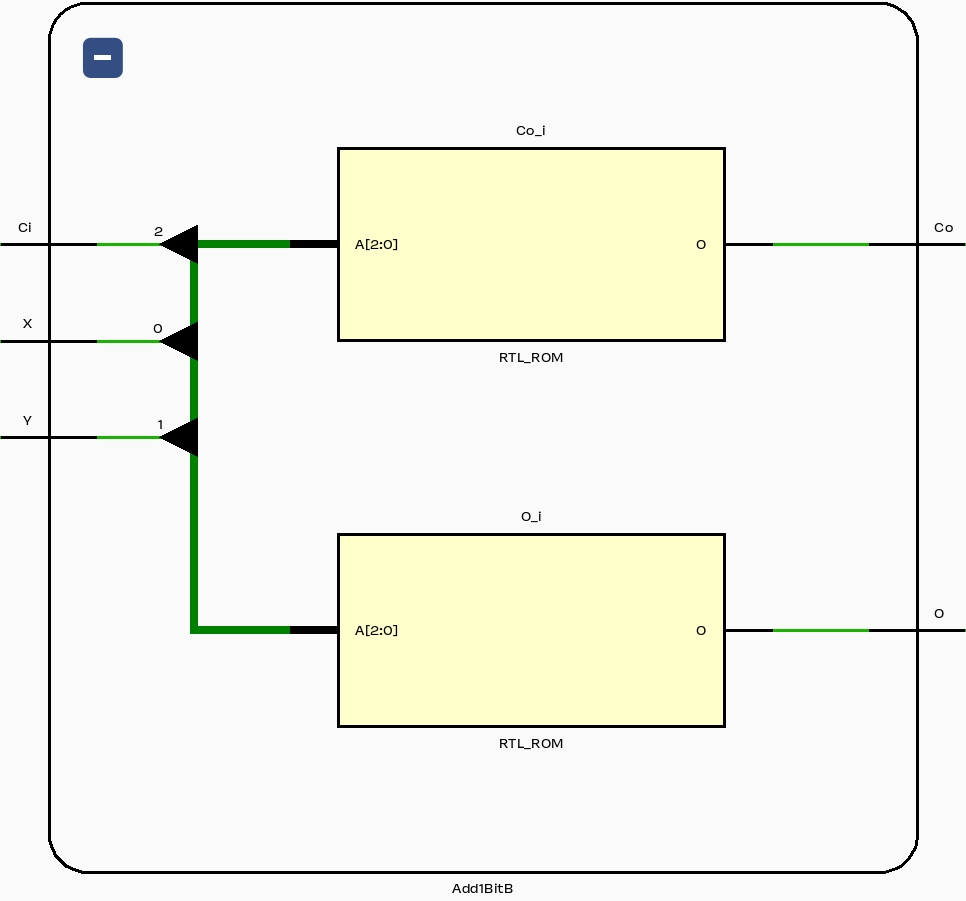
\includegraphics[width=.6\textwidth]{assets/img/schematic-add1bitb.png}
	\caption{Module Add1BitB}
\end{figure}


\newpage
\section{Tables de Vérité et Karnaugh}

% \begin{figure}[H]
% \centering
% \begin{karnaugh-map}[4][4][1][$D$][$C$][$B$][$A$]
% \manualterms{
% 	0,1,2,3,
% 	4,5,6,7,
% 	8,9,10,11,
% 	12,13,14,15}
% \implicant{2}{10}
% \implicant{4}{13}
% \implicant{12}{10}
% \implicantedge{3}{2}{11}{10}
% \end{karnaugh-map}
% \caption{TEMPLATE NOT GOOD}
% \end{figure}


\begin{table}[H]
	\centering
	\caption{Table de vérité des Bits}
	\label{tab:table-de-vérité-thermométrique-4-bits}
	\vspace{.2cm}
	\begin{tabular}{llllllll}
		\toprule
		A & B & C & D & E & F & G & H \\
		\midrule
		0 & 0 & 0 & 0 & 0 & 0 & 0 & 0 \\
		0 & 0 & 0 & 1 & 0 & 0 & 0 & 1 \\
		0 & 0 & 1 & 1 & 0 & 0 & 1 & 0 \\
		0 & 1 & 1 & 1 & 0 & 0 & 1 & 1 \\
		1 & 1 & 1 & 1 & 0 & 1 & 0 & 0 \\
		\bottomrule
	\end{tabular}

\end{table}

\begin{figure}[H]
\centering
\begin{karnaugh-map}[4][4][1][$D$][$C$][$B$][$A$]
\manualterms{
	0,1,X,0,
	X,X,X,1,
	X,X,X,X,
	X,X,X,0}
\implicant{1}{9}
\implicant{4}{6}
\end{karnaugh-map}
\caption{Karnaugh pour le bit $H$}
\label{tab:karnaugh-bit-H}
\end{figure}

\begin{figure}[H]
\centering
\begin{karnaugh-map}[4][4][1][$D$][$C$][$B$][$A$]
\manualterms{
	0,0,X,1,
	X,X,X,1,
	X,X,X,X,
	X,X,X,0}
\implicant{3}{6}
\end{karnaugh-map}
\caption{Karnaugh pour le bit $G$}
\label{tab:karnaugh-bit-G}
\end{figure}

\end{document}
